\documentclass[12pt]{tufte-book}
%DIF LATEXDIFF DIFFERENCE FILE
%DIF DEL notes-F24-old.tex   Wed Sep 18 19:45:02 2024
%DIF ADD notes-F24-new.tex   Wed Sep 18 19:44:44 2024
\usepackage{amsthm,amssymb,amsmath,thmtools,datetime,tikz}
\setcounter{secnumdepth}{3}

\declaretheorem[numberwithin=chapter,shaded={bgcolor=Lavender}]{definition}

\declaretheorem[numberwithin=chapter,shaded={bgcolor=Thistle}]{lemma}
\declaretheorem[numberwithin=chapter,shaded={bgcolor=Thistle}]{claim}

\declaretheorem[numberwithin=chapter,shaded={bgcolor=Apricot}]{theorem}

\declaretheorem[numberwithin=chapter,shaded={bgcolor=yellow}]{remark}
\declaretheorem[numberwithin=chapter]{exercise}
\declaretheorem[numberwithin=chapter,shaded={bgcolor=pink}]{construction}
\usepackage[
    type={CC},
    modifier={by-nc-nd},
    version={4.0},
]{doclicense}

\usepackage{graphicx,xcolor,mdframed}
%\usepackage[version=0.96]{pgf}
\usepackage{enumitem}

\def\chpcolor{blue!45}
\def\chpcolortxt{blue!60}

\iffalse
\titleformat{\chapter}%
  {\huge\rmfamily\itshape\color{red}}% format applied to label+text
  {\llap{\colorbox{red}{\parbox{1.5cm}{\hfill\itshape\huge\color{white}\thechapter}}}}% label
  {2pt}% horizontal separation between label and title body
  {}% before the title body
  []% after the title body
\fi

\hypersetup{colorlinks}% uncomment this line if you prefer colored hyperlinks (e.g., for onscreen viewing)

%%
% Book metadata
\title{A Course in Theory of Cryptography}
\author[Sanjam Garg]{Sanjam Garg}
%\publisher{Publisher of This Book}

%%
% If they're installed, use Bergamo and Chantilly from www.fontsite.com.
% They're clones of Bembo and Gill Sans, respectively.
%\IfFileExists{bergamo.sty}{\usepackage[osf]{bergamo}}{}% Bembo
%\IfFileExists{chantill.sty}{\usepackage{chantill}}{}% Gill Sans

%\usepackage{microtype}

%%
% Just some sample text
\usepackage{lipsum}
\newcommand{\ma}{\mathcal{A}}
%%
% For nicely typeset tabular material
\usepackage{booktabs}

\usepackage[n,advantage,operators,sets,adversary,landau,probability,notions,logic,ff,mm,primitives,events,complexity,oracles,asymptotics,keys]{cryptocode} 
%%
% For graphics / images
\usepackage{graphicx,algpseudocode}
\setkeys{Gin}{width=\linewidth,totalheight=\textheight,keepaspectratio}
\graphicspath{{graphics/}}

% The fancyvrb package lets us customize the formatting of verbatim
% environments.  We use a slightly smaller font.
\usepackage{fancyvrb}
\fvset{fontsize=\normalsize}

%%
% Prints argument within hanging parentheses (i.e., parentheses that take
% up no horizontal space).  Useful in tabular environments.
\newcommand{\hangp}[1]{\makebox[0pt][r]{(}#1\makebox[0pt][l]{)}}

%%
% Prints an asterisk that takes up no horizontal space.
% Useful in tabular environments.
\newcommand{\hangstar}{\makebox[0pt][l]{*}}

%%
% Prints a trailing space in a smart way.
\usepackage{xspace}

%%
% Some shortcuts for Tufte's book titles.  The lowercase commands will
% produce the initials of the book title in italics.  The all-caps commands
% will print out the full title of the book in italics.
\newcommand{\vdqi}{\textit{VDQI}\xspace}
\newcommand{\ei}{\textit{EI}\xspace}
\newcommand{\ve}{\textit{VE}\xspace}
\newcommand{\be}{\textit{BE}\xspace}
\newcommand{\VDQI}{\textit{The Visual Display of Quantitative Information}\xspace}
\newcommand{\EI}{\textit{Envisioning Information}\xspace}
\newcommand{\VE}{\textit{Visual Explanations}\xspace}
\newcommand{\BE}{\textit{Beautiful Evidence}\xspace}

\newcommand{\TL}{Tufte-\LaTeX\xspace}

% Prints the month name (e.g., January) and the year (e.g., 2008)
\newcommand{\monthyear}{%
  \ifcase\month\or January\or February\or March\or April\or May\or June\or
  July\or August\or September\or October\or November\or
  December\fi\space\number\year
}


% Prints an epigraph and speaker in sans serif, all-caps type.
\newcommand{\openepigraph}[2]{%
  %\sffamily\fontsize{14}{16}\selectfont
  \begin{fullwidth}
  \sffamily\large
  \begin{doublespace}
  \noindent\allcaps{#1}\\% epigraph
  \noindent\allcaps{#2}% author
  \end{doublespace}
  \end{fullwidth}
}

% Inserts a blank page
\newcommand{\blankpage}{\newpage\hbox{}\thispagestyle{empty}\newpage}

\usepackage{units}

% Typesets the font size, leading, and measure in the form of 10/12x26 pc.
\newcommand{\measure}[3]{#1/#2$\times$\unit[#3]{pc}}

% Macros for typesetting the documentation
\newcommand{\hlred}[1]{\textcolor{Maroon}{#1}}% prints in red
\newcommand{\hangleft}[1]{\makebox[0pt][r]{#1}}
\newcommand{\hairsp}{\hspace{1pt}}% hair space
\newcommand{\hquad}{\hskip0.5em\relax}% half quad space
\newcommand{\TODO}{\textcolor{red}{\bf TODO!}\xspace}
\newcommand{\ie}{\textit{i.\hairsp{}e.}\xspace}
\newcommand{\eg}{\textit{e.\hairsp{}g.}\xspace}
\newcommand{\na}{\quad--}% used in tables for N/A cells
\providecommand{\XeLaTeX}{X\lower.5ex\hbox{\kern-0.15em\reflectbox{E}}\kern-0.1em\LaTeX}
\newcommand{\tXeLaTeX}{\XeLaTeX\index{XeLaTeX@\protect\XeLaTeX}}
% \index{\texttt{\textbackslash xyz}@\hangleft{\texttt{\textbackslash}}\texttt{xyz}}
\newcommand{\tuftebs}{\symbol{'134}}% a backslash in tt type in OT1/T1
\newcommand{\doccmdnoindex}[2][]{\texttt{\tuftebs#2}}% command name -- adds backslash automatically (and doesn't add cmd to the index)
\newcommand{\doccmddef}[2][]{%
  \hlred{\texttt{\tuftebs#2}}\label{cmd:#2}%
  \ifthenelse{\isempty{#1}}%
    {% add the command to the index
      \index{#2 command@\protect\hangleft{\texttt{\tuftebs}}\texttt{#2}}% command name
    }%
    {% add the command and package to the index
      \index{#2 command@\protect\hangleft{\texttt{\tuftebs}}\texttt{#2} (\texttt{#1} package)}% command name
      \index{#1 package@\texttt{#1} package}\index{packages!#1@\texttt{#1}}% package name
    }%
}% command name -- adds backslash automatically
\newcommand{\doccmd}[2][]{%
  \texttt{\tuftebs#2}%
  \ifthenelse{\isempty{#1}}%
    {% add the command to the index
      \index{#2 command@\protect\hangleft{\texttt{\tuftebs}}\texttt{#2}}% command name
    }%
    {% add the command and package to the index
      \index{#2 command@\protect\hangleft{\texttt{\tuftebs}}\texttt{#2} (\texttt{#1} package)}% command name
      \index{#1 package@\texttt{#1} package}\index{packages!#1@\texttt{#1}}% package name
    }%
}% command name -- adds backslash automatically
\newcommand{\docopt}[1]{\ensuremath{\langle}\textrm{\textit{#1}}\ensuremath{\rangle}}% optional command argument
\newcommand{\docarg}[1]{\textrm{\textit{#1}}}% (required) command argument
\newenvironment{docspec}{\begin{quotation}\ttfamily\parskip0pt\parindent0pt\ignorespaces}{\end{quotation}}% command specification environment
\newcommand{\docenv}[1]{\texttt{#1}\index{#1 environment@\texttt{#1} environment}\index{environments!#1@\texttt{#1}}}% environment name
\newcommand{\docenvdef}[1]{\hlred{\texttt{#1}}\label{env:#1}\index{#1 environment@\texttt{#1} environment}\index{environments!#1@\texttt{#1}}}% environment name
\newcommand{\docpkg}[1]{\texttt{#1}\index{#1 package@\texttt{#1} package}\index{packages!#1@\texttt{#1}}}% package name
\newcommand{\doccls}[1]{\texttt{#1}}% document class name
\newcommand{\docclsopt}[1]{\texttt{#1}\index{#1 class option@\texttt{#1} class option}\index{class options!#1@\texttt{#1}}}% document class option name
\newcommand{\docclsoptdef}[1]{\hlred{\texttt{#1}}\label{clsopt:#1}\index{#1 class option@\texttt{#1} class option}\index{class options!#1@\texttt{#1}}}% document class option name defined
\newcommand{\docmsg}[2]{\bigskip\begin{fullwidth}\noindent\ttfamily#1\end{fullwidth}\medskip\par\noindent#2}
\newcommand{\docfilehook}[2]{\texttt{#1}\index{file hooks!#2}\index{#1@\texttt{#1}}}
\newcommand{\doccounter}[1]{\texttt{#1}\index{#1 counter@\texttt{#1} counter}}

% Generates the index
\usepackage{makeidx}
\makeindex
%DIF PREAMBLE EXTENSION ADDED BY LATEXDIFF
%DIF UNDERLINE PREAMBLE %DIF PREAMBLE
\RequirePackage[normalem]{ulem} %DIF PREAMBLE
\RequirePackage{color}\definecolor{RED}{rgb}{1,0,0}\definecolor{BLUE}{rgb}{0,0,1} %DIF PREAMBLE
\providecommand{\DIFadd}[1]{{\protect\color{blue}\uwave{#1}}} %DIF PREAMBLE
\providecommand{\DIFdel}[1]{{\protect\color{red}\sout{#1}}}                      %DIF PREAMBLE
%DIF SAFE PREAMBLE %DIF PREAMBLE
\providecommand{\DIFaddbegin}{} %DIF PREAMBLE
\providecommand{\DIFaddend}{} %DIF PREAMBLE
\providecommand{\DIFdelbegin}{} %DIF PREAMBLE
\providecommand{\DIFdelend}{} %DIF PREAMBLE
\providecommand{\DIFmodbegin}{} %DIF PREAMBLE
\providecommand{\DIFmodend}{} %DIF PREAMBLE
%DIF FLOATSAFE PREAMBLE %DIF PREAMBLE
\providecommand{\DIFaddFL}[1]{\DIFadd{#1}} %DIF PREAMBLE
\providecommand{\DIFdelFL}[1]{\DIFdel{#1}} %DIF PREAMBLE
\providecommand{\DIFaddbeginFL}{} %DIF PREAMBLE
\providecommand{\DIFaddendFL}{} %DIF PREAMBLE
\providecommand{\DIFdelbeginFL}{} %DIF PREAMBLE
\providecommand{\DIFdelendFL}{} %DIF PREAMBLE
\newcommand{\DIFscaledelfig}{0.5}
%DIF HIGHLIGHTGRAPHICS PREAMBLE %DIF PREAMBLE
\RequirePackage{settobox} %DIF PREAMBLE
\RequirePackage{letltxmacro} %DIF PREAMBLE
\newsavebox{\DIFdelgraphicsbox} %DIF PREAMBLE
\newlength{\DIFdelgraphicswidth} %DIF PREAMBLE
\newlength{\DIFdelgraphicsheight} %DIF PREAMBLE
% store original definition of \includegraphics %DIF PREAMBLE
\LetLtxMacro{\DIFOincludegraphics}{\includegraphics} %DIF PREAMBLE
\newcommand{\DIFaddincludegraphics}[2][]{{\color{blue}\fbox{\DIFOincludegraphics[#1]{#2}}}} %DIF PREAMBLE
\newcommand{\DIFdelincludegraphics}[2][]{% %DIF PREAMBLE
\sbox{\DIFdelgraphicsbox}{\DIFOincludegraphics[#1]{#2}}% %DIF PREAMBLE
\settoboxwidth{\DIFdelgraphicswidth}{\DIFdelgraphicsbox} %DIF PREAMBLE
\settoboxtotalheight{\DIFdelgraphicsheight}{\DIFdelgraphicsbox} %DIF PREAMBLE
\scalebox{\DIFscaledelfig}{% %DIF PREAMBLE
\parbox[b]{\DIFdelgraphicswidth}{\usebox{\DIFdelgraphicsbox}\\[-\baselineskip] \rule{\DIFdelgraphicswidth}{0em}}\llap{\resizebox{\DIFdelgraphicswidth}{\DIFdelgraphicsheight}{% %DIF PREAMBLE
\setlength{\unitlength}{\DIFdelgraphicswidth}% %DIF PREAMBLE
\begin{picture}(1,1)% %DIF PREAMBLE
\thicklines\linethickness{2pt} %DIF PREAMBLE
{\color[rgb]{1,0,0}\put(0,0){\framebox(1,1){}}}% %DIF PREAMBLE
{\color[rgb]{1,0,0}\put(0,0){\line( 1,1){1}}}% %DIF PREAMBLE
{\color[rgb]{1,0,0}\put(0,1){\line(1,-1){1}}}% %DIF PREAMBLE
\end{picture}% %DIF PREAMBLE
}\hspace*{3pt}}} %DIF PREAMBLE
} %DIF PREAMBLE
\LetLtxMacro{\DIFOaddbegin}{\DIFaddbegin} %DIF PREAMBLE
\LetLtxMacro{\DIFOaddend}{\DIFaddend} %DIF PREAMBLE
\LetLtxMacro{\DIFOdelbegin}{\DIFdelbegin} %DIF PREAMBLE
\LetLtxMacro{\DIFOdelend}{\DIFdelend} %DIF PREAMBLE
\DeclareRobustCommand{\DIFaddbegin}{\DIFOaddbegin \let\includegraphics\DIFaddincludegraphics} %DIF PREAMBLE
\DeclareRobustCommand{\DIFaddend}{\DIFOaddend \let\includegraphics\DIFOincludegraphics} %DIF PREAMBLE
\DeclareRobustCommand{\DIFdelbegin}{\DIFOdelbegin \let\includegraphics\DIFdelincludegraphics} %DIF PREAMBLE
\DeclareRobustCommand{\DIFdelend}{\DIFOaddend \let\includegraphics\DIFOincludegraphics} %DIF PREAMBLE
\LetLtxMacro{\DIFOaddbeginFL}{\DIFaddbeginFL} %DIF PREAMBLE
\LetLtxMacro{\DIFOaddendFL}{\DIFaddendFL} %DIF PREAMBLE
\LetLtxMacro{\DIFOdelbeginFL}{\DIFdelbeginFL} %DIF PREAMBLE
\LetLtxMacro{\DIFOdelendFL}{\DIFdelendFL} %DIF PREAMBLE
\DeclareRobustCommand{\DIFaddbeginFL}{\DIFOaddbeginFL \let\includegraphics\DIFaddincludegraphics} %DIF PREAMBLE
\DeclareRobustCommand{\DIFaddendFL}{\DIFOaddendFL \let\includegraphics\DIFOincludegraphics} %DIF PREAMBLE
\DeclareRobustCommand{\DIFdelbeginFL}{\DIFOdelbeginFL \let\includegraphics\DIFdelincludegraphics} %DIF PREAMBLE
\DeclareRobustCommand{\DIFdelendFL}{\DIFOaddendFL \let\includegraphics\DIFOincludegraphics} %DIF PREAMBLE
%DIF LISTINGS PREAMBLE %DIF PREAMBLE
\RequirePackage{listings} %DIF PREAMBLE
\RequirePackage{color} %DIF PREAMBLE
\lstdefinelanguage{DIFcode}{ %DIF PREAMBLE
%DIF DIFCODE_UNDERLINE %DIF PREAMBLE
  moredelim=[il][\color{red}\sout]{\%DIF\ <\ }, %DIF PREAMBLE
  moredelim=[il][\color{blue}\uwave]{\%DIF\ >\ } %DIF PREAMBLE
} %DIF PREAMBLE
\lstdefinestyle{DIFverbatimstyle}{ %DIF PREAMBLE
	language=DIFcode, %DIF PREAMBLE
	basicstyle=\ttfamily, %DIF PREAMBLE
	columns=fullflexible, %DIF PREAMBLE
	keepspaces=true %DIF PREAMBLE
} %DIF PREAMBLE
\lstnewenvironment{DIFverbatim}{\lstset{style=DIFverbatimstyle}}{} %DIF PREAMBLE
\lstnewenvironment{DIFverbatim*}{\lstset{style=DIFverbatimstyle,showspaces=true}}{} %DIF PREAMBLE
%DIF END PREAMBLE EXTENSION ADDED BY LATEXDIFF

\begin{document}
\iffalse
  % Front matter
  \frontmatter

  % r.1 blank page
  \blankpage


  % v.2 epigraphs
  \newpage\thispagestyle{empty}
  \openepigraph{%
    The public is more familiar with bad design than good design.
    It is, in effect, conditioned to prefer bad design,
    because that is what it lives with.
    The new becomes threatening, the old reassuring.
  }{Paul Rand%, {\itshape Design, Form, and Chaos}
  }
  \vfill
  \openepigraph{%
  A designer knows that he has achieved perfection
  not when there is nothing left to add,
  but when there is nothing left to take away.
  }{Antoine de Saint-Exup\'{e}ry}
  \vfill
  \openepigraph{%
    \ldots the designer of a new system must not only be the implementor and the first
    large-scale user; the designer should also write the first user manual\ldots
    If I had not participated fully in all these activities,
    literally hundreds of improvements would never have been made,
    because I would never have thought of them or perceived
    why they were important.
  }{Donald E. Knuth}
\fi

% r.3 full title page
\maketitle


% v.4 copyright page
%\newpage
\begin{fullwidth}
  ~\vfill
  \thispagestyle{empty}
  \setlength{\parindent}{0pt}
  \setlength{\parskip}{\baselineskip}
  Copyright \copyright\ \the\year\ \thanklessauthor

  %\par\smallcaps{Published by \thanklesspublisher}

  \par\smallcaps{This document is continually being updated. Please send us your feedback.}


  \par \doclicenseThis
  \index{license}

  \par\textit{This draft was compiled on \today.}
\end{fullwidth}

% r.5 contents
\tableofcontents

%\listoffigures

%\listoftables

% r.7 dedication
\iffalse
  \cleardoublepage
  ~\vfill

  \begin{doublespace}
    \noindent\fontsize{18}{22}\selectfont\itshape
    \nohyphenation
    Dedicated to those who appreciate \LaTeX{}
    and the work of \mbox{Edward R.~Tufte}
    and \mbox{Donald E.~Knuth}.
  \end{doublespace}
  \vfill
  \vfill

  % r.9 introduction
  \cleardoublepage
\fi
\chapter*{Preface}
Cryptography enables many paradoxical objects, such as public key encryption, verifiable electronic signatures, zero-knowledge protocols, and fully homomorphic encryption.  The two main steps in developing such seemingly impossible primitives are (i) defining the desired security properties formally and (ii) obtaining a construction satisfying the security property provably. In modern cryptography, the second step typically assumes (unproven) computational assumptions, which are conjectured to be computationally intractable. In this course, we will define several cryptographic primitives and argue their security based on well-studied computational hardness assumptions. However, we will largely ignore the mathematics underlying the assumed computational intractability assumptions.

\section*{Acknowledgements}
These lecture notes are based on scribe notes taken by students in CS 276 over the years. Also, thanks to Peihan Miao, Akshayaram Srinivasan, and Bhaskar Roberts for helping to improve these notes.
%%
% Start the main matter (normal chapters)
\newcommand{\sanjam}[1]{{\color{red} Sanjam: #1}}

\newcommand{\bhaskar}[1]{{\color{ForestGreen} Bhaskar: #1}}


\mainmatter
\section{Pseudorandom Functions}
In this section, we first define pseudorandom functions, and then show how to  construct a pseudorandom function from a pseudorandom generator.

Considering the set of all functions $f: \{0, 1\}^n \rightarrow \{0, 1\}^n$, there are $(2^n)^{2^n}$ of them.
To describe a random function in this set we need $n \cdot 2^n$ bits.
Intuitively, a pseudorandom function is one that cannot be distinguished from a random one,
but needs much fewer bits (e.g., polynomial in $n$) to be described.
Note that we restrict the distinguisher to only being allowed to ask the function poly($n$) times and decide whether it is random or pseudorandom.

\subsection{Definitions}

\begin{definition}[Function Ensemble]
    A \emph{function ensemble} is a sequence of random variables $F_1, F_2, \cdots, F_n, \cdots$ denoted as $\{F_n\}_{n \in \mathbb{N}}$ such that
    $F_n$ assumes values in the set of functions mapping $n$-bit input to $n$-bit output.
\end{definition}
\DIFaddbegin \DIFadd{Although we will only focus on the functions where the input and output bit-length is the same, the definition can be generalized to functions mapping \mbox{%DIFAUXCMD
$n$
}%DIFAUXCMD
-bit inputs to \mbox{%DIFAUXCMD
$m$
}%DIFAUXCMD
-bit outputs as \mbox{%DIFAUXCMD
$\{F_{n, m}\}_{n, m \in \mathbb{N}}$
}%DIFAUXCMD
.
}\DIFaddend 

\begin{definition}[Random Function Ensemble]
    We denote a random function ensemble by $\{R_n\}_{n \in \mathbb{N}}$.
\end{definition}
\DIFaddbegin \DIFadd{A sampling of the random variable \mbox{%DIFAUXCMD
$R_n$
}%DIFAUXCMD
requires \mbox{%DIFAUXCMD
$n \cdot 2^n$
}%DIFAUXCMD
bits to describe.
}\DIFaddend 

\begin{definition}[Efficiently Computable Function Ensemble]
    A function ensemble is called \emph{efficiently computable} if
    \begin{enumerate}[label=(\alph*)]
        \item \textbf{Succinct}:
              $\exists$ a PPT algorithm $I$ and a mapping $\phi$ from strings to functions such that
              $\phi(I(1^n))$ and $F_n$ are identically distributed.
              Note that we can view \DIFdelbegin \DIFdel{\mbox{%DIFAUXCMD
$I$
}%DIFAUXCMD
}\DIFdelend \DIFaddbegin \DIFadd{the output of \mbox{%DIFAUXCMD
$I(\cdot)$
}%DIFAUXCMD
}\DIFaddend as the description of the function.
        \item \textbf{Efficient}:
              $\exists$ a poly-time machine $V$ such that
              $V(i, x) = f_i(x)$ for every $x \in \{0, 1\}^n$, where $i$ is in the range of $I(1^n)$, and $f_i = \phi(i)$.
    \end{enumerate}
\end{definition}

\DIFaddbegin \DIFadd{Note that the succinctness condition implies that a sample from \mbox{%DIFAUXCMD
$F_n$
}%DIFAUXCMD
can be equivalently generated by first sampling a random string \mbox{%DIFAUXCMD
$k$
}%DIFAUXCMD
from \mbox{%DIFAUXCMD
$\{0, 1\}^n$
}%DIFAUXCMD
, and then outputting \mbox{%DIFAUXCMD
$f_k$
}%DIFAUXCMD
. Here \mbox{%DIFAUXCMD
$k$
}%DIFAUXCMD
is often called the ``key'' of the function}\footnote{\DIFadd{An efficiently computable function requires only \mbox{%DIFAUXCMD
$n$
}%DIFAUXCMD
bits (the key) to describe, while a random function requires \mbox{%DIFAUXCMD
$n.2^n$
}%DIFAUXCMD
bits.}}\DIFadd{. More generally, the key can be a string of length \mbox{%DIFAUXCMD
$m$
}%DIFAUXCMD
where \mbox{%DIFAUXCMD
$n$
}%DIFAUXCMD
is polynomial in \mbox{%DIFAUXCMD
$m$
}%DIFAUXCMD
; here \mbox{%DIFAUXCMD
$I$
}%DIFAUXCMD
uses a random tape of length \mbox{%DIFAUXCMD
$m$
}%DIFAUXCMD
and outputs \mbox{%DIFAUXCMD
$n$
}%DIFAUXCMD
bits. %DIF > However, we will only consider the case where the key is of length $n$.
}

\DIFaddend \begin{definition}[Pseudorandom Function Ensemble]
    A function ensemble $F = \{F_n\}_{n \in \mathbb{N}}$ is \emph{pseudorandom} if
    for every non-uniform PPT oracle adversary $\ma$, there exists a negligible function $\epsilon(n)$ such that
    \[
        \big| \Pr[\ma^{F_n} (1^n) = 1] - \Pr[\ma^{R_n} (1^n) = 1]  \big| \leq \epsilon(n).
    \]
    Here by saying ``oracle'' it means that $\ma$ has ``oracle access'' to a \DIFaddbegin \DIFadd{(fixed) }\DIFaddend function (in our definition, the function is \DIFaddbegin \DIFadd{a sampling of }\DIFaddend $F_n$ or $R_n$), and each call to that function costs 1 unit of time.
\end{definition}

Note that we will only consider efficiently computable pseudorandom ensembles in the following. \DIFaddbegin \DIFadd{Therefore, each function in \mbox{%DIFAUXCMD
$F_n$
}%DIFAUXCMD
is defined by a PRF key \mbox{%DIFAUXCMD
$k \in \{0, 1\}^n$
}%DIFAUXCMD
.
}\DIFaddend 


\subsection{Construction of PRF from PRG}

\begin{construction}
    Given a PRG $G: \{0, 1\}^n \rightarrow \{0, 1\}^{2n}$,
    let $G_0(x)$ be the first $n$ bits of $G(x)$, $G_1(x)$ be the last $n$ bits of $G(x)$.
    We construct $F^{(K)}: \{0, 1\}^n \rightarrow \{0, 1\}^n$ as follows.
    \[
        F^{(K)}_n(x_1 x_2 \cdots x_n) := G_{x_n}(G_{x_{n-1}} (\cdots(G_{x_1}(K)) \cdots  )),
    \]
    where $K \in \{0,1\}^n$ is the key to the pseudorandom function. \DIFdelbegin \DIFdel{Here \mbox{%DIFAUXCMD
$i$
}%DIFAUXCMD
is an \mbox{%DIFAUXCMD
$n$
}%DIFAUXCMD
-bit string, which is the seed of the pseudorandom function}\DIFdelend \DIFaddbegin \DIFadd{In Figure \ref{fig:binary-tree}, \mbox{%DIFAUXCMD
$i = K$
}%DIFAUXCMD
}\DIFaddend .
\end{construction}
The construction can be viewed as a binary tree of depth $n$, as shown in Figure \ref{fig:binary-tree}\DIFaddbegin \footnote{\DIFadd{Algorithmically, \mbox{%DIFAUXCMD
$F_n^{(K)}(x)$
}%DIFAUXCMD
is computed as:
}\begin{enumerate}
    \item \DIFadd{Set \mbox{%DIFAUXCMD
$y \gets K \in \{0, 1\}^n$
}%DIFAUXCMD
.
    }\item \DIFadd{For \mbox{%DIFAUXCMD
$i = 1 \dots n$
}%DIFAUXCMD
: update \mbox{%DIFAUXCMD
$y \gets G_{x_i}(y)$
}%DIFAUXCMD
.
    }\item \DIFadd{Output \mbox{%DIFAUXCMD
$y$
}%DIFAUXCMD
.
}\end{enumerate}
}\DIFaddend .

\begin{marginfigure}
    \centering
    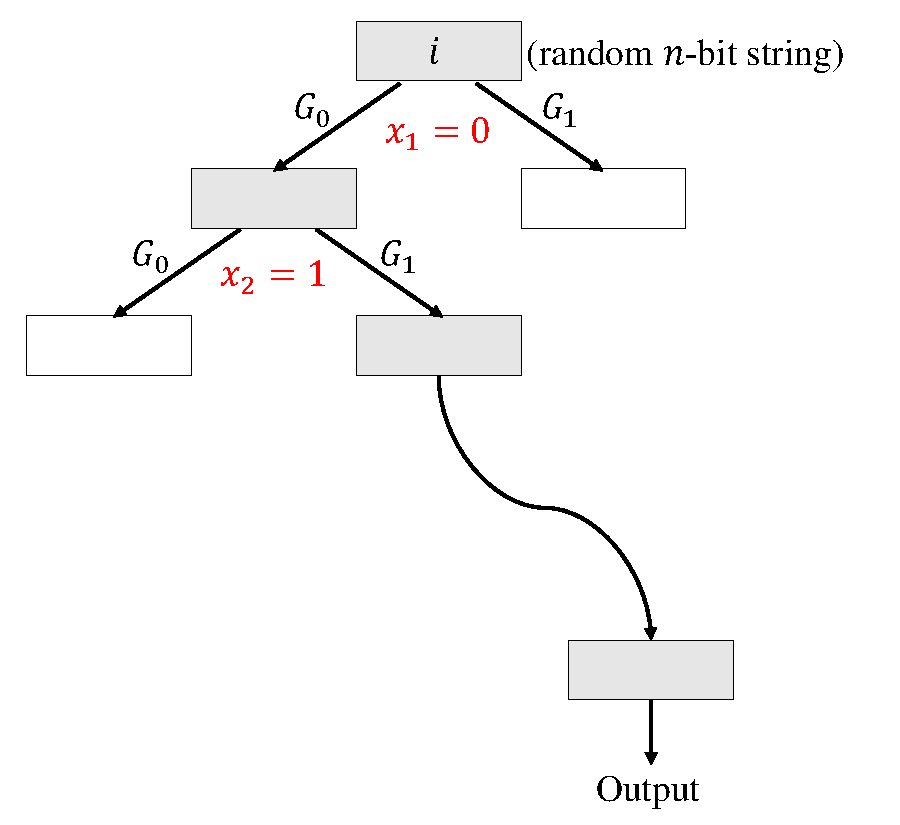
\includegraphics[width=\textwidth]{Old Scribe Notes/binary-tree.pdf}
    \caption{View the construction as a binary tree}
    \label{fig:binary-tree}
\end{marginfigure}

\begin{theorem}\label{theorem:ggm}
    The function ensemble $\{F_n\}_{n \in \mathbb{N}}$ constructed above is pseudorandom.
\end{theorem}

\proof
Assume for the sake of contradiction that $\{F_n\}_{n \in \mathbb{N}}$ is not \DIFdelbegin \DIFdel{PRG}\DIFdelend \DIFaddbegin \DIFadd{a PRF}\DIFaddend .
Then there exists a non-uniform PPT oracle adversary $\ma$ that can distinguish $\{F_n\}_{n \in \mathbb{N}}$ from $\{R_n\}_{n \in \mathbb{N}}$. Below, via a hybrid argument, we prove that this contradicts the fact that $G$ is a PRG\DIFaddbegin \DIFadd{; we will construct an adversary \mbox{%DIFAUXCMD
$\mathcal{B}$
}%DIFAUXCMD
that can distinguish between a sample from \mbox{%DIFAUXCMD
$U_{2n}$
}%DIFAUXCMD
and \mbox{%DIFAUXCMD
$G(U_{n})$
}%DIFAUXCMD
. We will prove for a fixed \mbox{%DIFAUXCMD
$n$
}%DIFAUXCMD
, and the proof can be easily extended to all \mbox{%DIFAUXCMD
$n \in \mathbb{N}$
}%DIFAUXCMD
}\DIFaddend .\DIFaddbegin \smallskip
\DIFaddend 

\DIFaddbegin \noindent \textbf{\DIFadd{Hybrids}}\DIFadd{. }\DIFaddend Consider the sequence of hybrids $H_i$ for $i \in \{ 0, 1, \cdots, n\}$ where the hybrid $i$ is defined as follows:
\[H\DIFdelbegin \DIFdel{_{n,i}^{(K)} }\DIFdelend \DIFaddbegin \DIFadd{_{i}^{(K_i)} }\DIFaddend (x_1x_2\ldots x_n ):= G_{x_n}(G_{x_{n-1}} (\cdots(G_{x_{i+1}}(K\DIFaddbegin \DIFadd{_i}\DIFaddend (x\DIFdelbegin \DIFdel{_i}\DIFdelend \DIFaddbegin \DIFadd{_1}\dots \DIFaddend x_{i-1}\DIFdelbegin \DIFdel{\ldots }\DIFdelend x\DIFdelbegin \DIFdel{_1}\DIFdelend \DIFaddbegin \DIFadd{_i}\DIFaddend ))) \cdots  )), \]
where \DIFdelbegin \DIFdel{\mbox{%DIFAUXCMD
$K$
}%DIFAUXCMD
}\DIFdelend \DIFaddbegin \DIFadd{\mbox{%DIFAUXCMD
$K_i$
}%DIFAUXCMD
}\DIFaddend is a random function from $\{0,1\}^{i}$ to $\{0,1\}^n$. Intuitively, hybrid $H_i$ corresponds to a binary tree of depth $n$ where the nodes of levels $0$ to $i$ correspond to random values and the nodes at levels $i+1$ to $n$ correspond to pseudorandom values. By inspection, observe that hybrids $H_0$ and $H_n$ are identical to a pseudorandom function and a random function, respectively. \DIFdelbegin \DIFdel{There it suffices to prove that hybrids }\DIFdelend \DIFaddbegin \DIFadd{Note that we cannot yet reduce the computational indistinguishability of }\DIFaddend $H_i$ and $H_{i+1}$ \DIFdelbegin \DIFdel{are computationally indistinguishable for each \mbox{%DIFAUXCMD
$i \in \{ 0, 1, \cdots, n\}$
}%DIFAUXCMD
.}\DIFdelend \DIFaddbegin \DIFadd{to security of the PRG \mbox{%DIFAUXCMD
$G$
}%DIFAUXCMD
because the adversary can make multiple oracle queries at different inputs.}\smallskip
\DIFaddend 

\DIFaddbegin \noindent \textbf{\DIFadd{Sub-hybrids}}\DIFadd{. }\DIFaddend We show that $H_{i}$ and $H_{i+1}$ are indistinguishable by considering a sequence of sub-hybrids $H_{i,j}$ for \DIFdelbegin \DIFdel{\mbox{%DIFAUXCMD
$j \in \{0,\ldots q_{i+1}\}$
}%DIFAUXCMD
, where \mbox{%DIFAUXCMD
$q_{i+1}$
}%DIFAUXCMD
}\DIFdelend \DIFaddbegin \DIFadd{\mbox{%DIFAUXCMD
$j \in \{0,\ldots q\}$
}%DIFAUXCMD
, where \mbox{%DIFAUXCMD
$q$
}%DIFAUXCMD
}\DIFaddend is the number of \DIFdelbegin \DIFdel{the distinct \mbox{%DIFAUXCMD
$i-bit$
}%DIFAUXCMD
prefixes of the queries of }\DIFdelend \DIFaddbegin \DIFadd{oracle queries made by }\DIFaddend $\mathcal{A}$\DIFaddbegin \footnote{\DIFadd{Observe that \mbox{%DIFAUXCMD
$\mathcal{A}$
}%DIFAUXCMD
can make at most polynomial in \mbox{%DIFAUXCMD
$n$
}%DIFAUXCMD
oracle queries. Looking ahead, our outer adversary \mbox{%DIFAUXCMD
$\mathcal{B}$
}%DIFAUXCMD
can either take \mbox{%DIFAUXCMD
$q$
}%DIFAUXCMD
as the max queries allowed to \mbox{%DIFAUXCMD
$\mathcal{A}$
}%DIFAUXCMD
, or guess the number, and double the guess each time if it's an under-estimate.}}\DIFadd{.
Intuitively, with each sub-hybrid \mbox{%DIFAUXCMD
$H_{i,j}$
}%DIFAUXCMD
, at level \mbox{%DIFAUXCMD
$i+1$
}%DIFAUXCMD
in the tree, we will fix the first \mbox{%DIFAUXCMD
$j$
}%DIFAUXCMD
oracle queries made by \mbox{%DIFAUXCMD
$\mathcal{A}$
}%DIFAUXCMD
to be output of random functions and the rest to be output of PRG. Let \mbox{%DIFAUXCMD
$R_i: \{0, 1\}^i \to \{0, 1\}^n$
}%DIFAUXCMD
and \mbox{%DIFAUXCMD
$S_{i}: \{0, 1\}^{i+1} \to \{0, 1\}^n$
}%DIFAUXCMD
be two random functions.
We define sub-hybrid \mbox{%DIFAUXCMD
$H_{i,j}^{(R_i, S_{i})}(x_1x_2\dots x_n)$
}%DIFAUXCMD
algorithmically as follows:
}\begin{enumerate}
    \item \DIFadd{Initialize a list \mbox{%DIFAUXCMD
$L \gets \{\}$
}%DIFAUXCMD
to store the \mbox{%DIFAUXCMD
$i$
}%DIFAUXCMD
-bit prefixes of the queries made by \mbox{%DIFAUXCMD
$\mathcal{A}$
}%DIFAUXCMD
}\DIFaddend .
    \DIFdelbegin \footnote{\DIFdel{Observe that \mbox{%DIFAUXCMD
$q_{i+1}$
}%DIFAUXCMD
for each appropriate choice of \mbox{%DIFAUXCMD
$i$
}%DIFAUXCMD
is bounded by the running time of \mbox{%DIFAUXCMD
$\mathcal{A}$
}%DIFAUXCMD
. Hence, this value is bounded by a polynomial in the security parameter.}}
%DIFAUXCMD
\addtocounter{footnote}{-1}%DIFAUXCMD
\DIFdelend \DIFaddbegin \item \DIFadd{If \mbox{%DIFAUXCMD
$|L| < j$
}%DIFAUXCMD
or \mbox{%DIFAUXCMD
$(x_1\dots x_i) \in L$
}%DIFAUXCMD
}\footnote{\DIFadd{Captures the first \mbox{%DIFAUXCMD
$j$
}%DIFAUXCMD
queries or any query with repeated \mbox{%DIFAUXCMD
$i$
}%DIFAUXCMD
-bit prefix to a previous query.}}\DIFadd{:
          }\begin{enumerate}[noitemsep,nolistsep]
              \item \DIFadd{Set \mbox{%DIFAUXCMD
$y \gets S_i(x_1\dots x_i x_{i+1})$
}%DIFAUXCMD
.
              }\item \DIFadd{Append \mbox{%DIFAUXCMD
$(x_1\dots x_i)$
}%DIFAUXCMD
to \mbox{%DIFAUXCMD
$L$
}%DIFAUXCMD
.
              }\item \DIFadd{For \mbox{%DIFAUXCMD
$a \in i+2 \dots n$
}%DIFAUXCMD
: update \mbox{%DIFAUXCMD
$y \gets G_{x_a}(y)$
}%DIFAUXCMD
.
          }\end{enumerate}
    \item \DIFadd{Else:
          }\begin{enumerate}[noitemsep,nolistsep]
              \item \DIFadd{Set \mbox{%DIFAUXCMD
$y \gets R_i(x_1\dots x_i)$
}%DIFAUXCMD
.
              }\item \DIFadd{For \mbox{%DIFAUXCMD
$a \in i+1 \dots n$
}%DIFAUXCMD
: update \mbox{%DIFAUXCMD
$y \gets G_{x_a}(y)$
}%DIFAUXCMD
.
          }\end{enumerate}
    \item \DIFadd{Output \mbox{%DIFAUXCMD
$y$
}%DIFAUXCMD
.
}\end{enumerate}
\DIFaddend 

\DIFdelbegin \DIFdel{We define hybrid \mbox{%DIFAUXCMD
$H_{i,j}$
}%DIFAUXCMD
for \mbox{%DIFAUXCMD
$j =0$
}%DIFAUXCMD
to be same as hybrid \mbox{%DIFAUXCMD
$H_{i}$
}%DIFAUXCMD
. Additionally, for \mbox{%DIFAUXCMD
$j >0$
}%DIFAUXCMD
hybrid \mbox{%DIFAUXCMD
$H_{i,j}$
}%DIFAUXCMD
is defined to be exactly the same as hybrid \mbox{%DIFAUXCMD
$H_{i,j-1}$
}%DIFAUXCMD
except the response provided to the attacker for the \mbox{%DIFAUXCMD
$j^{th}$
}%DIFAUXCMD
distinct \mbox{%DIFAUXCMD
$i-bit$
}%DIFAUXCMD
prefix query of \mbox{%DIFAUXCMD
$\mathcal{A}$
}%DIFAUXCMD
. Let this prefix be \mbox{%DIFAUXCMD
$x^*_n x^*_{n-1} \ldots x^*_{i}$
}%DIFAUXCMD
.
Note that in hybrid \mbox{%DIFAUXCMD
$H_{i,j-1}$
}%DIFAUXCMD
the children of the node \mbox{%DIFAUXCMD
$x^*_n x^*_{n-1} \ldots x^*_{i}$
}%DIFAUXCMD
correspond to two pseudorandom values.
              In hybrid \mbox{%DIFAUXCMD
$H_{i,j}$
}%DIFAUXCMD
we replace these two children with random values.
          By careful inspection, it follows that hybrid \mbox{%DIFAUXCMD
$H_{i,q_{i+1}}$
}%DIFAUXCMD
is actually }\DIFdelend \DIFaddbegin \DIFadd{Note that \mbox{%DIFAUXCMD
$H_{i, 0}$
}%DIFAUXCMD
is the same as \mbox{%DIFAUXCMD
$H_i$
}%DIFAUXCMD
and \mbox{%DIFAUXCMD
$H_{i, q}$
}%DIFAUXCMD
is the same as }\DIFaddend $H_{i+1}$. \DIFdelbegin \DIFdel{All we are left to prove is that hybrid \mbox{%DIFAUXCMD
$H_{i,j}$
}%DIFAUXCMD
and \mbox{%DIFAUXCMD
$H_{i,j+1}$
}%DIFAUXCMD
are indistinguishable for the appropriate choices of \mbox{%DIFAUXCMD
$j$
}%DIFAUXCMD
and we prove this below.}\DIFdelend \DIFaddbegin \DIFadd{Since we assumed that \mbox{%DIFAUXCMD
$\mathcal{A}$
}%DIFAUXCMD
can distinguish between \mbox{%DIFAUXCMD
$H_0$
}%DIFAUXCMD
and \mbox{%DIFAUXCMD
$H_n$
}%DIFAUXCMD
, by triangle inequality, there exists a \mbox{%DIFAUXCMD
$i^*, j^*$
}%DIFAUXCMD
such that it can distinguish \mbox{%DIFAUXCMD
$H_{i^*,j^*}$
}%DIFAUXCMD
and \mbox{%DIFAUXCMD
$H_{i^*,j^*+1}$
}%DIFAUXCMD
. We now focus on these two sub-hybrids}\footnote{\DIFadd{Looking ahead, the outer adversary \mbox{%DIFAUXCMD
$\mathcal{B}$
}%DIFAUXCMD
can guess \mbox{%DIFAUXCMD
$i^*, j^*$
}%DIFAUXCMD
; total choices are bounded by polynomial in \mbox{%DIFAUXCMD
$n$
}%DIFAUXCMD
. To simplify the proof, we will assume that \mbox{%DIFAUXCMD
$\mathcal{B}$
}%DIFAUXCMD
already knows this \mbox{%DIFAUXCMD
$i^*, j^*$
}%DIFAUXCMD
.}}\DIFadd{. Consider the \mbox{%DIFAUXCMD
$j^*+1$
}%DIFAUXCMD
-th query made by \mbox{%DIFAUXCMD
$\mathcal{A}$
}%DIFAUXCMD
(i.e. the first query where \mbox{%DIFAUXCMD
$|L|=j$
}%DIFAUXCMD
). Observe that this query cannot have the same \mbox{%DIFAUXCMD
$i$
}%DIFAUXCMD
-bit prefix as any of the previous queries. Because if it did, then the output distribution of the two hybrids would be identical, and that contradicts our assumption about \mbox{%DIFAUXCMD
$\mathcal{A}$
}%DIFAUXCMD
's distinguishing power. Therefore, the \mbox{%DIFAUXCMD
$j^*+1$
}%DIFAUXCMD
-th query has to be a new query, and this query is the only place where the two hybrids differ.}\smallskip
\DIFaddend 

\DIFaddbegin \noindent \textbf{\DIFadd{Outer adversary \mbox{%DIFAUXCMD
$\mathcal{B}$
}%DIFAUXCMD
}}\DIFadd{. }\DIFaddend Now we are ready to construct \DIFdelbegin \DIFdel{an }\DIFdelend \DIFaddbegin \DIFadd{our outer }\DIFaddend adversary $\mathcal{B}$ that \DIFdelbegin \DIFdel{distinguishes }\DIFdelend \DIFaddbegin \DIFadd{can distinguish between }\DIFaddend $U_{2n}$ \DIFdelbegin \DIFdel{from }\DIFdelend \DIFaddbegin \DIFadd{and }\DIFaddend $G(U_n)$\DIFdelbegin \DIFdel{: On input \mbox{%DIFAUXCMD
$T \in\{0, 1\}^{2n}$
}%DIFAUXCMD
(\mbox{%DIFAUXCMD
$T$
}%DIFAUXCMD
}\DIFdelend \DIFaddbegin \DIFadd{. \mbox{%DIFAUXCMD
$\mathcal{B}^{\mathcal{A}, i^*, j^*}(1^n, z)$
}%DIFAUXCMD
, where \mbox{%DIFAUXCMD
$z \in \{0, 1\}^{2n}$
}%DIFAUXCMD
(\mbox{%DIFAUXCMD
$z$
}%DIFAUXCMD
}\DIFaddend could be either from $U_{2n}$ or $G(U_n)$) \DIFdelbegin \DIFdel{,
construct a full binary tree of depth \mbox{%DIFAUXCMD
$n$
}%DIFAUXCMD
that is exactly the same as \mbox{%DIFAUXCMD
$H_{i,j}$
}%DIFAUXCMD
except replacing the children of  \mbox{%DIFAUXCMD
$x^*_n x^*_{n-1} \ldots x^*_{i}$
}%DIFAUXCMD
by the value \mbox{%DIFAUXCMD
$T$
}%DIFAUXCMD
.
              Observe that the only difference between \mbox{%DIFAUXCMD
$H_{i,j}$
}%DIFAUXCMD
and \mbox{%DIFAUXCMD
$H_{i,j+1}$
}%DIFAUXCMD
is that values corresponding to nodes \mbox{%DIFAUXCMD
$x_n^*\ldots x_i^* 0$
}%DIFAUXCMD
and \mbox{%DIFAUXCMD
$x_n^*\ldots x_i^* 1$
}%DIFAUXCMD
are pseudorandom or random respectively. }\DIFdelend \DIFaddbegin \DIFadd{and we assume the knowledge of \mbox{%DIFAUXCMD
$i^*, j^*$
}%DIFAUXCMD
}\footnote{\DIFadd{As mentioned before, it can be guessed with slight loss in distinguishing advantage.}}\DIFadd{, operates as follows:
}\begin{enumerate}
    \item \DIFadd{Parse \mbox{%DIFAUXCMD
$z$
}%DIFAUXCMD
as \mbox{%DIFAUXCMD
$z_0||z_1$
}%DIFAUXCMD
, where \mbox{%DIFAUXCMD
$z_0, z_1 \in \{0, 1\}^n$
}%DIFAUXCMD
.
    }\item \DIFadd{For all the oracle queries from \mbox{%DIFAUXCMD
$\mathcal{A}$
}%DIFAUXCMD
except the \mbox{%DIFAUXCMD
$j^*+1$
}%DIFAUXCMD
-th query, respond as \mbox{%DIFAUXCMD
$H_{i^*,j^*}$
}%DIFAUXCMD
}\footnote{\DIFadd{The outer adversary \mbox{%DIFAUXCMD
$\mathcal{B}$
}%DIFAUXCMD
runs a random function in polynomial time in \mbox{%DIFAUXCMD
$n$
}%DIFAUXCMD
via lazy sampling. It generates a random output on a new input and caches responses to previous inputs.}}\DIFadd{.
    }\item \DIFadd{For the \mbox{%DIFAUXCMD
$j^*+1$
}%DIFAUXCMD
-th query \mbox{%DIFAUXCMD
$(x_1\dots x_n)$
}%DIFAUXCMD
, do the following:
          }\begin{enumerate}
              \item \DIFadd{Set \mbox{%DIFAUXCMD
$y \gets z_{x_{i^*+1}}$
}%DIFAUXCMD
.
              }\item \DIFadd{For \mbox{%DIFAUXCMD
$a \in i^*+2 \dots n$
}%DIFAUXCMD
: update \mbox{%DIFAUXCMD
$y \gets G_{x_a}(y)$
}%DIFAUXCMD
.
              }\item \DIFadd{Respond with \mbox{%DIFAUXCMD
$y$
}%DIFAUXCMD
.
          }\end{enumerate}
    \item \DIFadd{Output whatever \mbox{%DIFAUXCMD
$\mathcal{A}$
}%DIFAUXCMD
outputs.
}\end{enumerate}

\DIFadd{We assumed that \mbox{%DIFAUXCMD
$\mathcal{A}$
}%DIFAUXCMD
can distinguish between \mbox{%DIFAUXCMD
$H_{i^*, j^*}$
}%DIFAUXCMD
and \mbox{%DIFAUXCMD
$H_{i^*, j^*+1}$
}%DIFAUXCMD
, so by contrapositive of the Sunglass Lemma, }\DIFaddend $\mathcal{B}$ \DIFdelbegin \DIFdel{uses the value \mbox{%DIFAUXCMD
$T$
}%DIFAUXCMD
to generate these two nodes. Hence success in  distinguishing hybrids \mbox{%DIFAUXCMD
$H_{i,j}$
}%DIFAUXCMD
and \mbox{%DIFAUXCMD
$H_{i,j+1}$
}%DIFAUXCMD
provides a successful attack for \mbox{%DIFAUXCMD
$\mathcal{B}$
}%DIFAUXCMD
in violating security of the pseudorandom generator.
}\DIFdelend \DIFaddbegin \DIFadd{can distinguish between \mbox{%DIFAUXCMD
$U_{2n}$
}%DIFAUXCMD
and \mbox{%DIFAUXCMD
$G(U_n)$
}%DIFAUXCMD
. This contradicts that \mbox{%DIFAUXCMD
$G$
}%DIFAUXCMD
is a PRG.
}

%DIF > where $q_{i+1}$ is the number of the distinct $i-bit$ prefixes of the queries of $\mathcal{A}$.\footnote{Observe that $q_{i+1}$ for each appropriate choice of $i$ is bounded by the running time of $\mathcal{A}$. Hence, this value is bounded by a polynomial in the security parameter.}
%DIF > We define hybrid $H_{i,j}$ for $j =0$ to be same as hybrid $H_{i}$. Additionally, for $j >0$ hybrid $H_{i,j}$ is defined to be exactly the same as hybrid $H_{i,j-1}$ except the response provided to the attacker for the $j^{th}$ distinct $i-bit$ prefix query of $\mathcal{A}$. Let this prefix be $x^*_n x^*_{n-1} \ldots x^*_{i}$. Note that in hybrid $H_{i,j-1}$ the children of the node $x^*_n x^*_{n-1} \ldots x^*_{i}$ correspond to two pseudorandom values. In hybrid $H_{i,j}$ we replace these two children with random values. By careful inspection, it follows that hybrid $H_{i,q_{i+1}}$ is actually $H_{i+1}$. All we are left to prove is that hybrid $H_{i,j}$ and $H_{i,j+1}$ are indistinguishable for the appropriate choices of $j$ and we prove this below.
%DIF > Now we are ready to construct an adversary $\mathcal{B}$ that  distinguishes $U_{2n}$ from $G(U_n)$: On input $T \in\{0, 1\}^{2n}$ ($T$ could be either from $U_{2n}$ or $G(U_n)$),
%DIF > construct a full binary tree of depth $n$ that is exactly the same as $H_{i,j}$ except replacing the children of  $x^*_n x^*_{n-1} \ldots x^*_{i}$ by the value $T$.
%DIF > Observe that the only difference between $H_{i,j}$ and $H_{i,j+1}$ is that values corresponding to nodes $x_n^*\ldots x_i^* 0$ and $x_n^*\ldots x_i^* 1$ are pseudorandom or random respectively. $\mathcal{B}$ uses the value $T$ to generate these two nodes. Hence success in  distinguishing hybrids $H_{i,j}$ and $H_{i,j+1}$ provides a successful attack for $\mathcal{B}$ in violating security of the pseudorandom generator.
\DIFaddend \qed







\section{PRFs from DDH: Naor-Reingold PRF}
We will now describe a PRF function family $F_n: \mathcal{K} \times \{0,1\}^n \rightarrow \mathbb{G}_n$ where DDH is assumed to be hard for  $\{\mathbb{G}_n\}$ and $\mathcal{K}$ is the key space.
The \DIFdelbegin \DIFdel{seed }\DIFdelend \DIFaddbegin \DIFadd{key }\DIFaddend for the PRF $F_n$ will be $K =  (h, u_1, \ldots u_n)$, where $u,u_0\ldots u_n$ are sampled uniformly from $|\mathbb{G}_n|$, $g$ is the generator of $\mathbb{G}_n$ and $h = g^u$. \DIFaddbegin \DIFadd{Compared to the previous construction (Theorem~\ref{theorem:ggm}), there are two differences to note already: the key is polynomially longer and the output space is \mbox{%DIFAUXCMD
$\mathbb{G}_n$
}%DIFAUXCMD
instead of \mbox{%DIFAUXCMD
$\{0, 1\}^n$
}%DIFAUXCMD
.
}\DIFaddend 

\[F_n(K,x) = h^{\prod_{i} u_i^{x_i}}\]

Next, we will prove that the function $F_n$ is a pseudo-random function or that $\{F_n\}$ is a pseudo-random function ensemble.\footnote{Here, we require that adversary distinguish the function $F_n$ from a random function from $\{0,1\}^n$ to $\mathbb{G}_n$. Note that the output range of the function is $\mathbb{G}_n$. \DIFdelbegin \DIFdel{Note }\DIFdelend \DIFaddbegin \DIFadd{Moreover, note }\DIFaddend that the distribution of random group elements in $\mathbb{G}_n$ might actually be far from uniformly random strings.}
\begin{lemma}
    Assuming the DDH Assumption (see Definition~\ref{def:ddh}) for $\{\mathbb{G}_n\}$ is hard, we have that $\{F_n\}$ is a pseudorandom function ensemble.
\end{lemma}
\begin{proof}
    The proof of this lemma is similar to the proof of Theorem~\ref{theorem:ggm} \DIFaddbegin \DIFadd{except for some subtle differences that arise from number theory}\footnote{\DIFadd{At a high-level, we can no longer fix nodes in the same level of the tree arbitrarily. Fixing one node has implications for how other nodes will be changed. This is because we have a fixed basis in the key.}}\DIFaddend .

    Let \DIFdelbegin \DIFdel{\mbox{%DIFAUXCMD
$R_n^j$
}%DIFAUXCMD
}\DIFdelend \DIFaddbegin \DIFadd{\mbox{%DIFAUXCMD
$R_n$
}%DIFAUXCMD
}\DIFaddend be random function from \DIFdelbegin \DIFdel{\mbox{%DIFAUXCMD
$\{0,1\}^j \rightarrow \mathbb{G}_n$
}%DIFAUXCMD
}\DIFdelend \DIFaddbegin \DIFadd{\mbox{%DIFAUXCMD
$\{0,1\}^n \rightarrow \mathbb{G}_n$
}%DIFAUXCMD
}\DIFaddend . Then we want to prove that for all non-uniform PPT adversaries $\mathcal{A}$ we have that:
    \[\mu(n) = \left|\Pr[\mathcal{A}^{F_n}(1^n) =1] -  \DIFdelbegin \DIFdel{\Pr[\mathcal{A}^{R_n^n}(1^n) =1]}\DIFdelend \DIFaddbegin \DIFadd{\Pr[\mathcal{A}^{R_n}(1^n) =1]}\DIFaddend \right|\]
    is a negligible function. \DIFaddbegin \smallskip
\DIFaddend 

    \DIFaddbegin \noindent \textbf{\DIFadd{Hybrids}}\DIFadd{. }\DIFaddend For the sake of contradiction, we assume that the function $F_n$ is not pseudorandom. Next, towards a contradiction, we consider a sequence of hybrid functions \DIFdelbegin \DIFdel{\mbox{%DIFAUXCMD
$F_n^0 \ldots F_n^n$
}%DIFAUXCMD
.
    For any \mbox{%DIFAUXCMD
$j \in \{0,\ldots n\}$
}%DIFAUXCMD
, let \mbox{%DIFAUXCMD
$F^j_n((h,u_{j}\ldots u_n),x) = (R_n^j(x_1\ldots x_j))^{\prod_{i=j+1}^n u_i^{x_i}}$
}%DIFAUXCMD
, where \mbox{%DIFAUXCMD
$R_n^0(\epsilon)$
}%DIFAUXCMD
}\DIFdelend \DIFaddbegin \DIFadd{\mbox{%DIFAUXCMD
$H^0_n \ldots H^n_n$
}%DIFAUXCMD
.
    For \mbox{%DIFAUXCMD
$j \in \{0, \dots, n\}$
}%DIFAUXCMD
, let \mbox{%DIFAUXCMD
$S^j_n: \{0, 1\}^j \to \{0, 1, \dots, |\mathbb{G}_n|-1\}$
}%DIFAUXCMD
, then hybrid \mbox{%DIFAUXCMD
$H_n^j$
}%DIFAUXCMD
is defined as}\footnote{\DIFadd{Algorithmically, \mbox{%DIFAUXCMD
$H_n^j((u,u_{j+1}\ldots u_n),x)$
}%DIFAUXCMD
is computed as:
    }\begin{enumerate}
        \item \DIFadd{Set \mbox{%DIFAUXCMD
$y \gets S_n^j(x_1\ldots x_j)$
}%DIFAUXCMD
.
        }\item \DIFadd{For \mbox{%DIFAUXCMD
$i = j+1 \dots n$
}%DIFAUXCMD
: update \mbox{%DIFAUXCMD
$y \gets y \cdot u_i^{x_i}$
}%DIFAUXCMD
.
        }\item \DIFadd{Output \mbox{%DIFAUXCMD
$g^y$
}%DIFAUXCMD
.
    }\end{enumerate}

    }\DIFadd{:
    }\begin{equation*}
        \DIFadd{H_n^j((u,u_{j+1}\ldots u_n),x) = \big(g^{S_n^j(x_1\ldots x_j)}\big)^{\prod_{i=j+1}^n u_i^{x_i}}
    }\end{equation*}
    \DIFadd{where \mbox{%DIFAUXCMD
$S_n^0(\cdot)$
}%DIFAUXCMD
}\DIFaddend is the constant function with output \DIFdelbegin \DIFdel{\mbox{%DIFAUXCMD
$h$
}%DIFAUXCMD
}\DIFdelend \DIFaddbegin \DIFadd{\mbox{%DIFAUXCMD
$u$
}%DIFAUXCMD
}\DIFaddend . Observe that \DIFdelbegin \DIFdel{\mbox{%DIFAUXCMD
$F_n^0$
}%DIFAUXCMD
}\DIFdelend \DIFaddbegin \DIFadd{\mbox{%DIFAUXCMD
$H_n^0$
}%DIFAUXCMD
}\DIFaddend is the same as the function $F_n$ and \DIFdelbegin \DIFdel{\mbox{%DIFAUXCMD
$F_n^n$
}%DIFAUXCMD
}\DIFdelend \DIFaddbegin \DIFadd{\mbox{%DIFAUXCMD
$H_n^n$
}%DIFAUXCMD
}\DIFaddend is the same as the function \DIFdelbegin \DIFdel{\mbox{%DIFAUXCMD
$R_n^n$
}%DIFAUXCMD
}\DIFdelend \DIFaddbegin \DIFadd{\mbox{%DIFAUXCMD
$R_n$
}%DIFAUXCMD
}\footnote{\DIFadd{A uniform group element is equivalently sampled by first sampling an exponent in the order of the group.}}\DIFaddend . Thus, by a hybrid argument \DIFaddbegin \DIFadd{and triangle inequality}\DIFaddend , we conclude that there exists \DIFdelbegin \DIFdel{\mbox{%DIFAUXCMD
$k \in \{0,\ldots n-1\}$
}%DIFAUXCMD
}\DIFdelend \DIFaddbegin \DIFadd{\mbox{%DIFAUXCMD
$j^* \in \{0,\ldots n-1\}$
}%DIFAUXCMD
}\DIFaddend , such that
    \[\left|\DIFdelbegin \DIFdel{\Pr[\mathcal{A}^{F_n^k}(1^n) =1] }\DIFdelend \DIFaddbegin \DIFadd{\Pr[\mathcal{A}^{H_n^{j^*}}(1^n) =1] }\DIFaddend -  \DIFdelbegin \DIFdel{\Pr[\mathcal{A}^{F_n^{k+1}}(1^n) =1]}\DIFdelend \DIFaddbegin \DIFadd{\Pr[\mathcal{A}^{H_n^{j^*+1}}(1^n) =1]}\DIFaddend \right|\]
    is a non-negligible function. Now all we are left to show is that this implies an attacker that refutes the DDH assumption.\DIFaddbegin \smallskip

    \noindent \textbf{\DIFadd{Sub-hybrids}}\DIFadd{. }\DIFaddend The proof of this claim follows by a sequence of \DIFdelbegin \DIFdel{\mbox{%DIFAUXCMD
$T$
}%DIFAUXCMD
}\DIFdelend \DIFaddbegin \DIFadd{\mbox{%DIFAUXCMD
$q+1$
}%DIFAUXCMD
}\DIFaddend sub-hybrids \DIFdelbegin \DIFdel{, where \mbox{%DIFAUXCMD
$T$
}%DIFAUXCMD
is the }\DIFdelend \DIFaddbegin \DIFadd{\mbox{%DIFAUXCMD
$H_n^{j, 0}, \dots, H_n^{j, q}$
}%DIFAUXCMD
, where \mbox{%DIFAUXCMD
$q$
}%DIFAUXCMD
is the (polynomially bounded by \mbox{%DIFAUXCMD
$n$
}%DIFAUXCMD
) }\DIFaddend running time of $\mathcal{A}$. \DIFdelbegin \DIFdel{Without loss of generality we assume that }\DIFdelend \DIFaddbegin \DIFadd{For the simplicity of exposition, we abuse the notation and denote \mbox{%DIFAUXCMD
$q(n)$
}%DIFAUXCMD
by \mbox{%DIFAUXCMD
$q$
}%DIFAUXCMD
. Let \mbox{%DIFAUXCMD
$C_n^j: \{0, 1\}^j \to \{0, \dots, |\mathbb{G}_n|-1\}$
}%DIFAUXCMD
and \mbox{%DIFAUXCMD
$D_n^j: \{0, 1\}^{j+1} \to \{0, \dots, |\mathbb{G}_n|-1\}$
}%DIFAUXCMD
be two random functions, and \mbox{%DIFAUXCMD
$C_n^0(\cdot) = u$
}%DIFAUXCMD
. We define sub-hybrid \mbox{%DIFAUXCMD
$H_n^{j, k}\big((u, u_{j+1}\ldots u_n),(x_1\dots x_n)\big)$
}%DIFAUXCMD
for \mbox{%DIFAUXCMD
$k \in \{0, \dots, q\}$
}%DIFAUXCMD
as follows:
    }\begin{enumerate}
        \item \DIFadd{Initialize a list \mbox{%DIFAUXCMD
$L \gets \{\}$
}%DIFAUXCMD
to store the \mbox{%DIFAUXCMD
$j$
}%DIFAUXCMD
-bit prefixes of the queries made by }\DIFaddend $\mathcal{A}$\DIFdelbegin \DIFdel{never makes the same query twice. }\DIFdelend \DIFaddbegin \DIFadd{.
        }\item \DIFadd{If \mbox{%DIFAUXCMD
$|L|<k$
}%DIFAUXCMD
or \mbox{%DIFAUXCMD
$(x_1\cdots x_j) \in L$
}%DIFAUXCMD
:
              }\begin{enumerate}[noitemsep,nolistsep]
                  \item \DIFadd{Set \mbox{%DIFAUXCMD
$y \gets D^j_n(x_1\dots x_{j+1})$
}%DIFAUXCMD
.
                  }\item \DIFadd{Append \mbox{%DIFAUXCMD
$(x_1\dots x_j)$
}%DIFAUXCMD
to \mbox{%DIFAUXCMD
$L$
}%DIFAUXCMD
.
                  }\item \DIFadd{For \mbox{%DIFAUXCMD
$i = j+2 \dots n$
}%DIFAUXCMD
: update \mbox{%DIFAUXCMD
$y \gets y \cdot u_i^{x_i}$
}%DIFAUXCMD
.
              }\end{enumerate}
        \item \DIFadd{Else
              }\begin{enumerate}[noitemsep,nolistsep]
                  \item \DIFadd{Set \mbox{%DIFAUXCMD
$y \gets C^j_n(x_1\dots x_j)$
}%DIFAUXCMD
.
                  }\item \DIFadd{For \mbox{%DIFAUXCMD
$i = j+1 \dots n$
}%DIFAUXCMD
: update \mbox{%DIFAUXCMD
$y \gets y \cdot u_i^{x_i}$
}%DIFAUXCMD
.
              }\end{enumerate}
        \item \DIFadd{Output \mbox{%DIFAUXCMD
$g^y$
}%DIFAUXCMD
.
    }\end{enumerate}
\DIFaddend 

    \DIFdelbegin \DIFdel{More specifically, we consider a sequence of functions \mbox{%DIFAUXCMD
$F_n^{k,t}$
}%DIFAUXCMD
where \mbox{%DIFAUXCMD
$t \in \{0,T\}$
}%DIFAUXCMD
, \mbox{%DIFAUXCMD
$F_n^{k,0}$
}%DIFAUXCMD
is same as \mbox{%DIFAUXCMD
$F_n^{k}$
}%DIFAUXCMD
and \mbox{%DIFAUXCMD
$F_n^{k,T}$
}%DIFAUXCMD
is same as \mbox{%DIFAUXCMD
$F_n^{k+1}$
}%DIFAUXCMD
.
    In particular, we explain how \mbox{%DIFAUXCMD
$F_n^{k,t}$
}%DIFAUXCMD
answers queries by }\DIFdelend \DIFaddbegin \DIFadd{It is easy to see that \mbox{%DIFAUXCMD
$H_n^{j, 0}$
}%DIFAUXCMD
is the same as \mbox{%DIFAUXCMD
$H_n^j$
}%DIFAUXCMD
and \mbox{%DIFAUXCMD
$H_n^{j, q}$
}%DIFAUXCMD
is the same as \mbox{%DIFAUXCMD
$H_n^{j+1}$
}%DIFAUXCMD
.
    Again, we use hybrid argument to conclude that there exists \mbox{%DIFAUXCMD
$j^*, k^*$
}%DIFAUXCMD
such that }\DIFaddend $\mathcal{A}$ \DIFdelbegin \DIFdel{.}\footnote{\DIFdel{As assumed earlier, keep in mind that \mbox{%DIFAUXCMD
$\mathcal{A}$
}%DIFAUXCMD
never makes the same query twice.}} %DIFAUXCMD
\addtocounter{footnote}{-1}%DIFAUXCMD
\DIFdel{Let \mbox{%DIFAUXCMD
$x^1, \ldots x^t$
}%DIFAUXCMD
be the first \mbox{%DIFAUXCMD
$t$
}%DIFAUXCMD
queries }\DIFdelend \DIFaddbegin \DIFadd{can distinguish between \mbox{%DIFAUXCMD
$H_n^{j^*, k^*}$
}%DIFAUXCMD
and \mbox{%DIFAUXCMD
$H_n^{j^*, k^*+1}$
}%DIFAUXCMD
with non-negligible probability. We now focus on these two sub-hybrids. Consider the \mbox{%DIFAUXCMD
$k^*+1$
}%DIFAUXCMD
-th oracle query }\DIFaddend made by $\mathcal{A}$. \DIFdelbegin \DIFdel{For any query , \mbox{%DIFAUXCMD
$x$
}%DIFAUXCMD
}\DIFdelend \DIFaddbegin \DIFadd{Following an identical argument we used in the proof of Theorem~\ref{theorem:ggm}, this query cannot be a repeat of a query made before, and this query is the only place where the two sub-hybrids differ.}\smallskip

    \noindent \textbf{\DIFadd{Outer adversary \mbox{%DIFAUXCMD
$\mathcal{B}$
}%DIFAUXCMD
}}\DIFadd{. The construction of the outer adversary \mbox{%DIFAUXCMD
$\mathcal{B}$
}%DIFAUXCMD
is a bit different from the proof of Theorem~\ref{theorem:ggm}. Intuitively, unlike Theorem~\ref{theorem:ggm}, outer adversary cannot simply replace the \mbox{%DIFAUXCMD
$k^*+1$
}%DIFAUXCMD
-th query with the DDH challenge in isolation from the rest of the queries }\DIFaddend made by $\mathcal{A}$\DIFdelbegin \DIFdel{such that the first \mbox{%DIFAUXCMD
$k$
}%DIFAUXCMD
bits of \mbox{%DIFAUXCMD
$x$
}%DIFAUXCMD
match the first \mbox{%DIFAUXCMD
$k$
}%DIFAUXCMD
bits of one of \mbox{%DIFAUXCMD
$x_1, \ldots x_y$
}%DIFAUXCMD
answer as \mbox{%DIFAUXCMD
$F_n^{k+1}$
}%DIFAUXCMD
else answer as \mbox{%DIFAUXCMD
$F_n^{k}$
}%DIFAUXCMD
.
              Now we can conclude that there exists a \mbox{%DIFAUXCMD
$t$
}%DIFAUXCMD
such that \mbox{%DIFAUXCMD
$F_n^{k,t}$
}%DIFAUXCMD
}\DIFdelend \DIFaddbegin \DIFadd{. This is because the pseudorandom nodes in the tree are tied together by the DDH relation, and are not independent, i.e., all pseudorandom sibling nodes on the same level of the tree are set apart by a common exponent.
}

    \DIFadd{\mbox{%DIFAUXCMD
$\mathcal{B}$
}%DIFAUXCMD
gets as challenge either a DDH tuple \mbox{%DIFAUXCMD
$(g, A=g^a, B=g^b, C=g^{ab})$
}%DIFAUXCMD
or a uniform tuple \mbox{%DIFAUXCMD
$(g, A=g^a, B=g^b, C=g^c)$
}%DIFAUXCMD
where \mbox{%DIFAUXCMD
$a, b, c$
}%DIFAUXCMD
are uniform in \mbox{%DIFAUXCMD
$\{0, \dots, |\mathbb{G}|-1\}$
}%DIFAUXCMD
. We construct \mbox{%DIFAUXCMD
$\mathcal{B}^{\mathcal{A}, j^*, k^*}\big(1^n, (g, A, B, C)\big)$
}%DIFAUXCMD
as follows:
    }\begin{enumerate}
        \item \DIFadd{Sample \mbox{%DIFAUXCMD
$u, u_{j^*+1}, \ldots u_n$
}%DIFAUXCMD
uniformly from \mbox{%DIFAUXCMD
$\{0, \dots, |\mathbb{G}_n|-1\}$
}%DIFAUXCMD
.
        }\item \DIFadd{For first \mbox{%DIFAUXCMD
$k^*$
}%DIFAUXCMD
queries from \mbox{%DIFAUXCMD
$\mathcal{A}$
}%DIFAUXCMD
, respond as \mbox{%DIFAUXCMD
$H_n^{j^*, k^*}((u, u_{j^*+1}, \ldots u_n),\cdot)$
}%DIFAUXCMD
.
        }\item \DIFadd{For the \mbox{%DIFAUXCMD
$k^*+1$
}%DIFAUXCMD
-th query \mbox{%DIFAUXCMD
$(x_1\ldots x_n)$
}%DIFAUXCMD
, do the following:
              }\begin{enumerate}[noitemsep,nolistsep]
                  \item \DIFadd{Set \mbox{%DIFAUXCMD
$y \gets A$
}%DIFAUXCMD
if \mbox{%DIFAUXCMD
$x_{j^*+1} = 0$
}%DIFAUXCMD
}\DIFaddend and \DIFdelbegin \DIFdel{\mbox{%DIFAUXCMD
$F_n^{k,t+1}$
}%DIFAUXCMD
are distinguishable with non-negligible probability. }\DIFdelend \DIFaddbegin \DIFadd{\mbox{%DIFAUXCMD
$y \gets C$
}%DIFAUXCMD
if \mbox{%DIFAUXCMD
$x_{j^*+1} = 1$
}%DIFAUXCMD
.
                  }\item \DIFadd{For \mbox{%DIFAUXCMD
$i = j^*+2 \dots n$
}%DIFAUXCMD
: update \mbox{%DIFAUXCMD
$y \gets y \cdot u_i^{x_i}$
}%DIFAUXCMD
.
                  }\item \DIFadd{Output \mbox{%DIFAUXCMD
$g^y$
}%DIFAUXCMD
.
              }\end{enumerate}
        \item \DIFadd{For the rest of the queries \mbox{%DIFAUXCMD
$(x_1\ldots x_n)$
}%DIFAUXCMD
, do the following:
              }\begin{enumerate}[noitemsep,nolistsep]
                  \item \DIFadd{Set \mbox{%DIFAUXCMD
$y \gets C^j_n(x_1\ldots x_j)$
}%DIFAUXCMD
.
                  }\item \DIFadd{For \mbox{%DIFAUXCMD
$i = j^*+2 \dots n$
}%DIFAUXCMD
: update \mbox{%DIFAUXCMD
$y \gets y \cdot u_i^{x_i}$
}%DIFAUXCMD
.
                  }\item \DIFadd{If \mbox{%DIFAUXCMD
$x_{j^*+1} = 0$
}%DIFAUXCMD
, output \mbox{%DIFAUXCMD
$g^y$
}%DIFAUXCMD
, else output}\footnote{\DIFadd{Recall that \mbox{%DIFAUXCMD
$B=g^b$
}%DIFAUXCMD
, so \mbox{%DIFAUXCMD
$B^y = g^{y\cdot b} = g^{y\cdot b^x_{j^*+1}}$
}%DIFAUXCMD
. Therefore, the DDH relation is properly set for all pseudorandom nodes.}} \DIFadd{\mbox{%DIFAUXCMD
$B^y$
}%DIFAUXCMD
.
              }\end{enumerate}
        \item \DIFadd{Output whatever \mbox{%DIFAUXCMD
$\mathcal{A}$
}%DIFAUXCMD
outputs.
    }\end{enumerate}
\DIFaddend 

    \DIFdelbegin \DIFdel{Finally, we will show that using an adversary that }\DIFdelend \DIFaddbegin \DIFadd{By the construction of \mbox{%DIFAUXCMD
$\mathcal{B}$
}%DIFAUXCMD
, if \mbox{%DIFAUXCMD
$(g, A, B, C)$
}%DIFAUXCMD
is a DDH tuple, then the distribution of oracle responses seen by \mbox{%DIFAUXCMD
$\mathcal{A}$
}%DIFAUXCMD
are exactly the same as the responses seen in the hybrid \mbox{%DIFAUXCMD
$H_n^{j^*, k^*}$
}%DIFAUXCMD
. Otherwise, they are the same as hybrid \mbox{%DIFAUXCMD
$H_n^{j^*, k^*+1}$
}%DIFAUXCMD
.
    We assumed that \mbox{%DIFAUXCMD
$\mathcal{A}$
}%DIFAUXCMD
}\DIFaddend can distinguish between \DIFdelbegin \DIFdel{\mbox{%DIFAUXCMD
$F_n^{k,t}$
}%DIFAUXCMD
and \mbox{%DIFAUXCMD
$F_n^{k,t+1}$
}%DIFAUXCMD
we need to construct an adversary }\DIFdelend \DIFaddbegin \DIFadd{\mbox{%DIFAUXCMD
$H_n^{j^*, k^*}$
}%DIFAUXCMD
and \mbox{%DIFAUXCMD
$H_n^{j^*, k^*+1}$
}%DIFAUXCMD
, therefore }\DIFaddend $\mathcal{B}$ \DIFdelbegin \DIFdel{that refutes the DDH assumption. We leave construction of this adversary as an exercise.
}\DIFdelend \DIFaddbegin \DIFadd{can distinguish between a DDH tuple and a uniform tuple. This contradicts our assumption that DDH is hard.
}

    %DIF > Without loss of generality we assume that $\mathcal{A}$ never makes the same query twice.
    %DIF > More specifically, we consider a sequence of functions $F_n^{k,t}$ where $t \in \{0,T\}$, $F_n^{k,0}$ is same as $F_n^{k}$ and $F_n^{k,T}$ is same as $F_n^{k+1}$. In particular, we explain how $F_n^{k,t}$ answers queries by $\mathcal{A}$.\footnote{As assumed earlier, keep in mind that $\mathcal{A}$ never makes the same query twice.} Let $x^1, \ldots x^t$ be the first $t$ queries made by $\mathcal{A}$. For any query, $x$ made by $\mathcal{A}$ such that the first $k$ bits of $x$ match the first $k$ bits of one of $x_1, \ldots x_y$ answer as $F_n^{k+1}$ else answer as $F_n^{k}$. Now we can conclude that there exists a $t$ such that $F_n^{k,t}$ and $F_n^{k,t+1}$ are distinguishable with non-negligible probability.
    %DIF > Finally, we will show that using an adversary that can distinguish between $F_n^{k,t}$ and $F_n^{k,t+1}$ we need to construct an adversary $\mathcal{B}$ that refutes the DDH assumption. We leave construction of this adversary as an exercise.
\DIFaddend \end{proof}


\newpage
\section*{Exercises}
\begin{exercise}
    \newcommand{\bit}{\{0,1\}}

    Prove or disprove: If $f$ is a one-way function, then the following function $B:\bit^*\to\bit$ is a hardconcentrate predicate for $f$. The function $B(x)$ outputs the inner product modulo 2 of the first $\lfloor |x|/2\rfloor$ bits of $x$ and the last $\lfloor |x|/2\rfloor$ bits of $x$.
\end{exercise}

\begin{exercise}
    Let $\phi(n)$ denote the first $n$ digits of $\pi = 3.141592653589\ldots$ after the decimal in binary ($\pi$ in its binary notation looks like $11.00100100001111110110101010001000100001\ldots$).

    Prove the following: if one-way functions exist, then there exists a one-way function $f$ such that the function $B:\{0,1\}^* \rightarrow \{0,1\}$ is not a hard concentrate bit of $f$. The function $B(x)$ outputs $\langle x, \phi(|x|)\rangle$, where
    \[\langle a, b\rangle := \sum_{i=1}^n a_i b_i \mod 2\]
    for the bit-representation of $a = {a_1a_2\cdots a_n}$ and $b= {b_1b_2\cdots b_n}$.
\end{exercise}

\begin{exercise}
    If $f: \{0,1\}^{n}\times \{0,1\}^n\rightarrow \{0,1\}^n$  is PRF, then in which of the following cases is $g: \{0,1\}^{n}\times \{0,1\}^n\rightarrow \{0,1\}^n$ also a PRF? \begin{enumerate} \item $g(K,x) = f(K,f(K,x))$ \item $g(K,x) = f(x,f(K,x))$ \item $g(K,x) = f(K,f(x,K))$
    \end{enumerate}
\end{exercise}

\begin{exercise}[Puncturable PRFs.] Puncturable PRFs are PRFs for which a key can be given out such that, it allows evaluation of the PRF on all inputs, except for one designated input.

    %\newcommand{\negl}{\mathsf{negl}}
    \newcommand{\A}{\mathcal{A}}
    \newcommand{\F}{F}
    \newcommand{\KeyF}{\mathsf{Key}_{\F}}
    \newcommand{\PunctureF}{\mathsf{Puncture}_{\F}}
    \newcommand{\EvalF}{\mathsf{Eval}_{\F}}


    A puncturable pseudo-random function $\F$ is given by a triple of efficient algorithms ($\KeyF$,$\PunctureF$, and $\EvalF$), satisfying the following conditions:
    \begin{itemize}
        \item[-] \textbf{Functionality preserved under puncturing}: For every $x^*, x \in \{0,1\}^{n}$ such that $x^* \neq x$, we have that:
              $$\Pr[\EvalF(K,x) = \EvalF(K_{x^*},x) : K \gets \KeyF(1^n), K_{x^*} = \PunctureF(K,x^*)] = 1$$
        \item[-] \textbf{Pseudorandom at the punctured point}: For every $x^*\in \{0,1\}^n$ we have that for every polysize adversary $\A$ we have that:
              $$|\Pr[\A(K_{x^*}, \EvalF(K,x^*)) = 1] - \Pr[\A(K_{x^*}, \EvalF(K,U_n)) = 1]|= \negl(n)$$
              where $K \gets \KeyF(1^n)$ and $K_S = \PunctureF(K,x^*)$. $U_n$ denotes the uniform distribution over $n$ bits.
    \end{itemize}

    Prove that: If one-way functions exist, then there exists a puncturable PRF family that maps $n$ bits to $n$ bits. \\
    \textbf{Hint:} The GGM tree-based construction of PRFs from a length doubling pseudorandom generator (discussed in class) can be adapted to construct a puncturable PRF. Also note that $K$ and $K_{x^*}$ need not be the same length.
\end{exercise}
%
%\subsection{Application}
%Consider an interesting game: Alice and Bob are talking on the phone.
%Alice flips a coin, and Bob guesses whether it's head or tail.
%But the problem is how can Alice convince Bob that the coin is indeed head or tail?
%If we have pseudorandom functions, the problem could be easily solved.
%
%Assume we have a PRF $F_n: \{0, 1\}^n \rightarrow \{0, 1\}^n$.
%Alice and Bob have a shared key $i \in \{0, 1\}^n$, then $f_i(\cdot)$ is shared information.
%Now Alice has a message $m \in \{0, 1\}^n$ and wants to let Bob guess it,
%the procedure consists of three steps.
%\begin{enumerate}[(a)]
%    \item Alice chooses a string $r \in \{0, 1\}^n$, and sends to Bob  $m' = f_i(r) \oplus m$ ;
%    \item Bob guesses $m$;
%    \item Alice sends $r$ to Bob.
%\end{enumerate}
%In step (a), since $F_n$ is PRF, all the information that Bob gets is a random $n$-bit string, so it will not influence his behavior in step (b).
%Then in step (c), Bob receives $r$ and will be convinced that the true value of $m$ is $f_i(r) \oplus m'$.
%


%%
% The back matter contains appendices, bibliographies, indices, glossaries, etc.



\backmatter

\DIFaddbegin \bibliography{cryptobib/abbrev0,cryptobib/crypto}
\DIFaddend \bibliographystyle{plainnat}


%\printindex
\end{document}
